%%%%%%%%%%%%%%%%%%%%%%%
%
% © Pierre-Louis Gstalter
% 02/16/2022
%
%%%%%%%%%%%%%%%%%%%%%%%
\documentclass{article}
\usepackage[left=1cm, right=1cm, top=1.5cm, bottom=1cm]{geometry}
\usepackage{multicol}
\usepackage{color}
\usepackage{graphicx}
\usepackage{hyperref}
\setlength{\columnseprule}{0pt}
\def\columnseprulecolor{\color{blue}}
\pagestyle{empty}

\begin{document}
\begin{multicols}{3}

Paris, France

pierre-louis.gstalter@minesparis.psl.eu

\texttt{+33647437563}

plgstalter.org

github.com/plgstalter

\columnbreak

	\hfill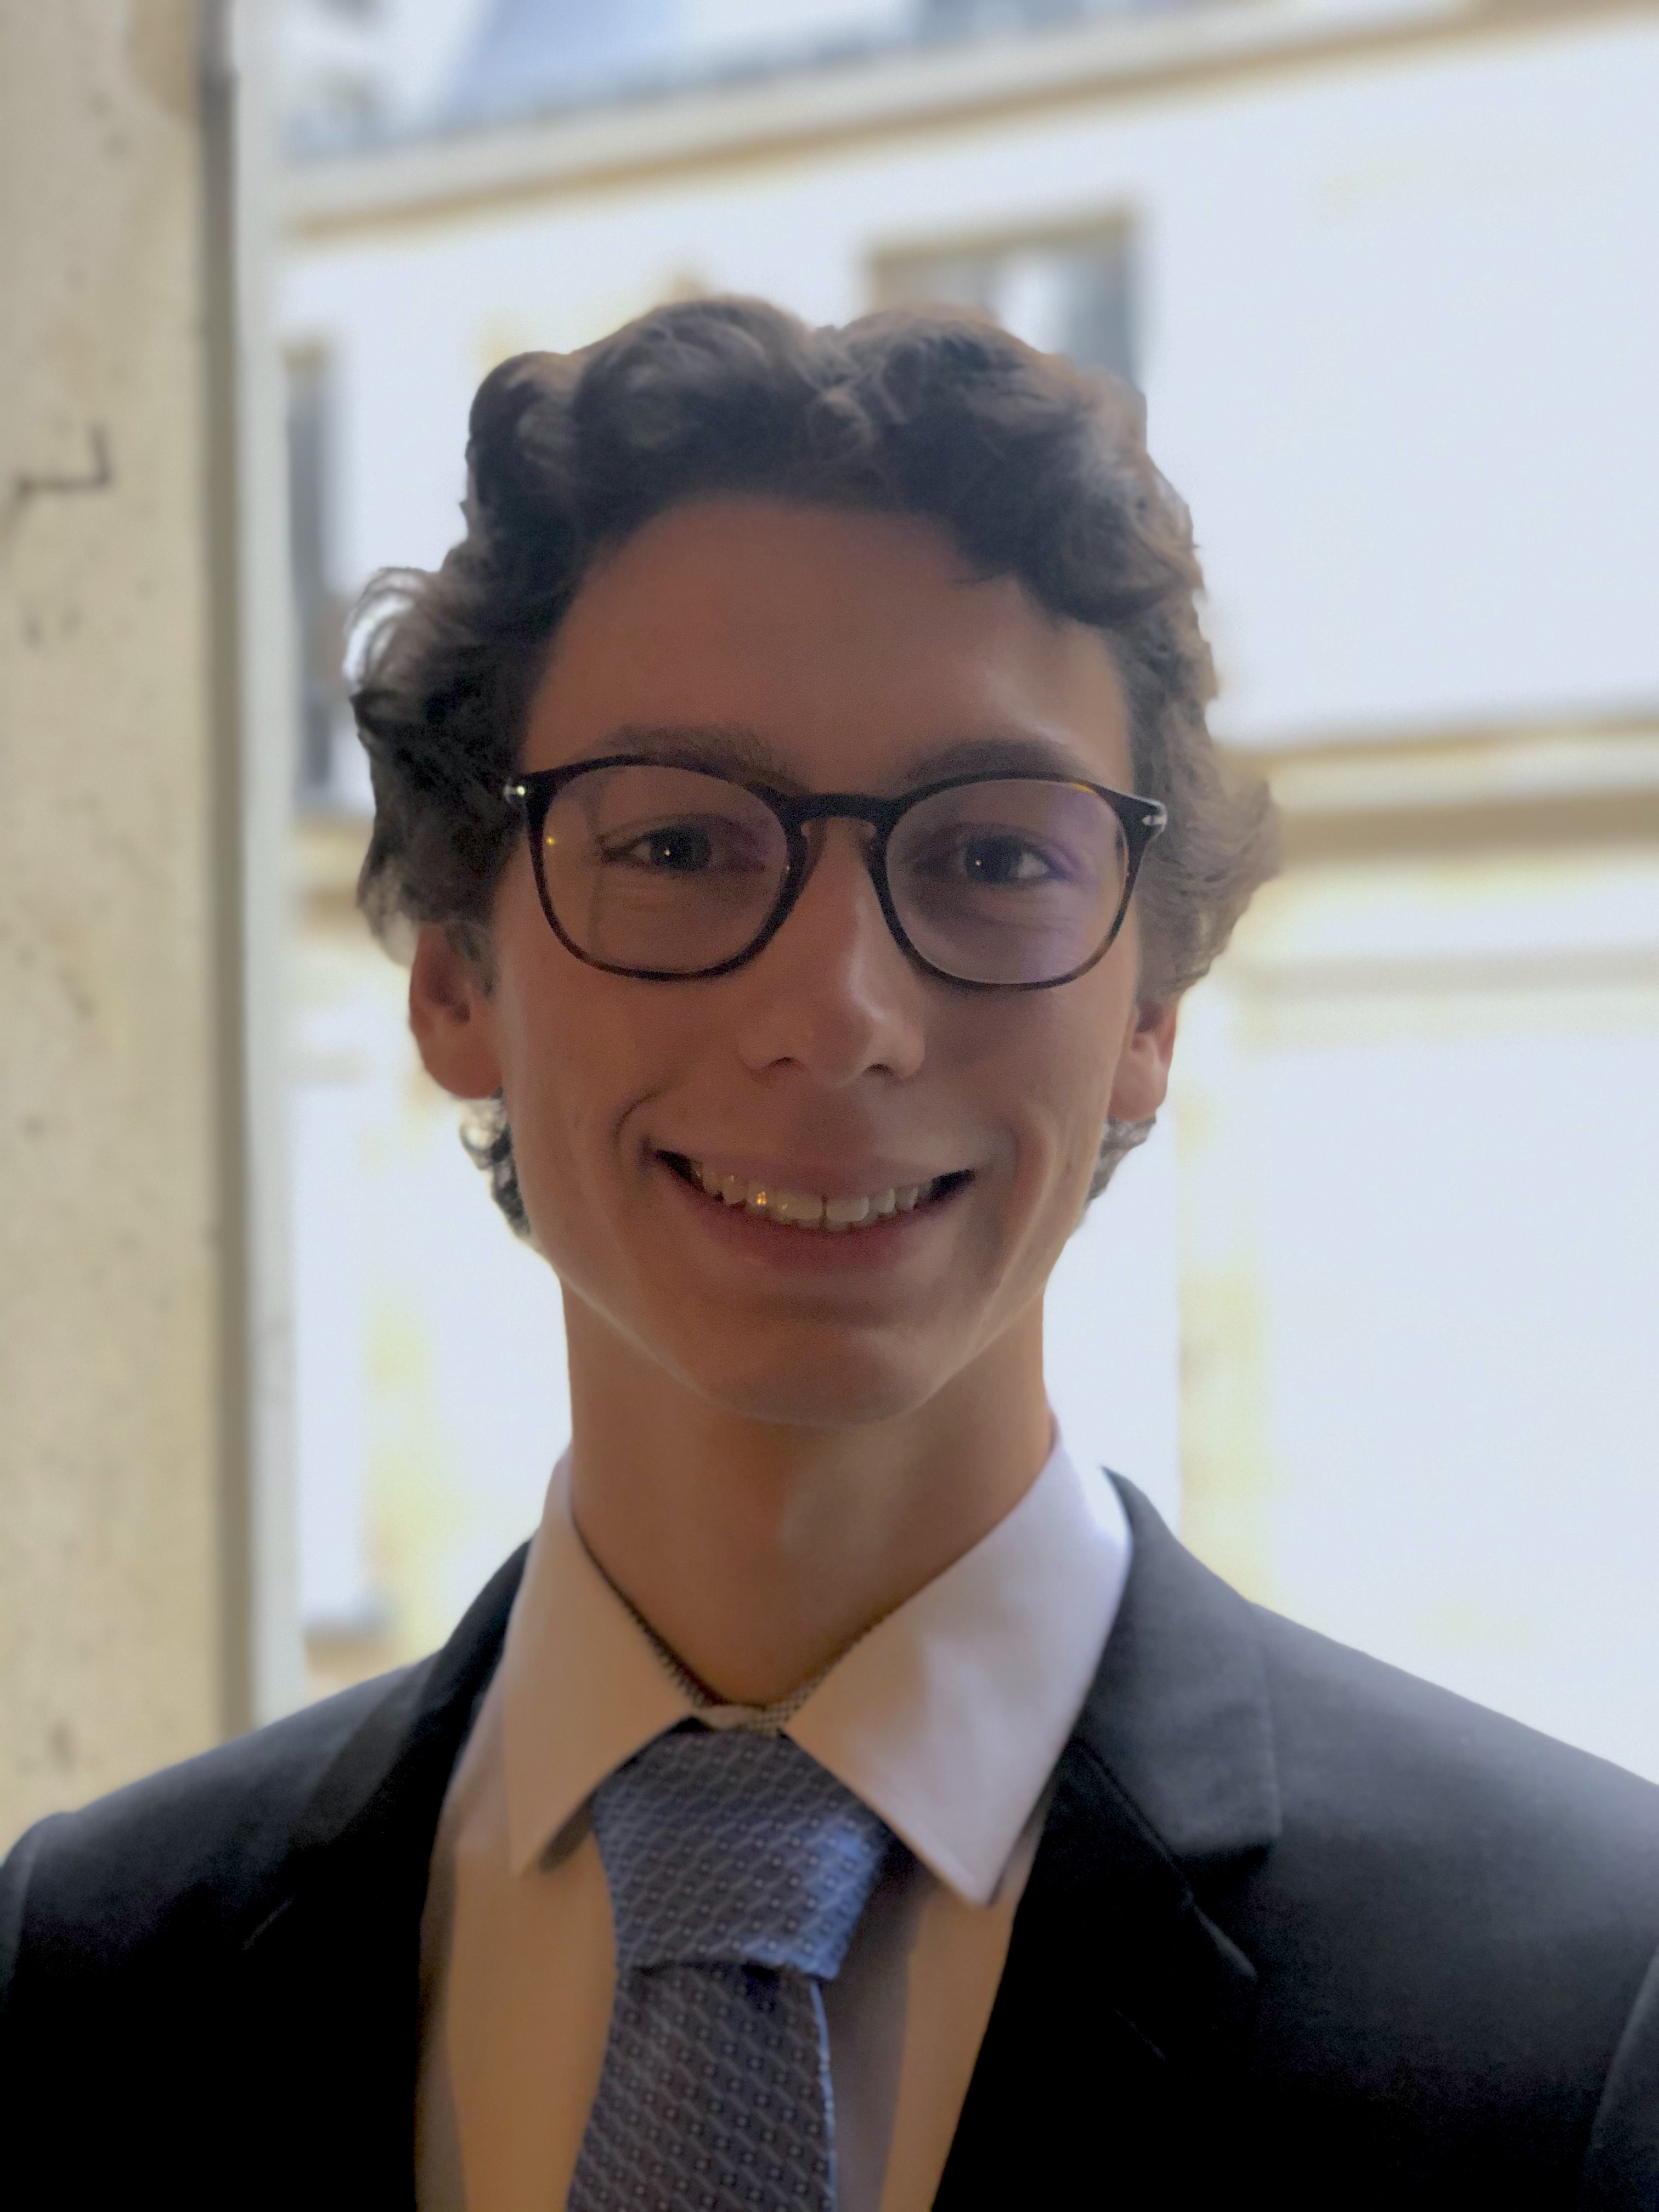
\includegraphics[width=2.6cm]{photo.jpeg}

\columnbreak

{\color{blue} \section*{Pierre-Louis Gstalter}}

\noindent Second Year student at Mines Paris, among France's top engineering schools. Fond of mathematics and computing, I'm looking for an internship in finance.
\end{multicols}

\setlength{\columnsep}{2cm}
\setlength{\columnseprule}{1.5pt}
\begin{multicols}{2}
	{\color{blue} \subsection*{Education}}

		\noindent\texttt{2020-2024} \textbf{Mines de Paris}

		\textbf{Mathematics: } probabilities, optimization,

		statistics, algebra

		\textbf{Computer science : } data analysis, object-oriented

		programming

\hfill

		\noindent\texttt{2021-2022} \textbf{Università degli Studi di Milano}

		Erasmus+ exchange, courses in English and Italian

		Financial mathematics, heuristic algorithms,

		combinatorial optimization

\hfill

		\noindent\texttt{2018-2020} \textbf{Lycée Henri IV}
		
		\textit{Classes Préparatoires aux Grandes Écoles}, highly 

		competitive mathematics and physics courses 

		preparing for France's best engineering schools

\hfill

	{\color{blue} \subsection*{Working Experience}}

		\noindent\texttt{02/2022-?} \textbf{Mathematics oral examiner}

		Lycée Henri IV, Paris


		\noindent\texttt{09/2020-?} \textbf{Personal teacher}

		Mathematics and physics courses, from high-school to 

		undergraduate level

\hfill
	
		\noindent\texttt{05/2021} \textbf{Sports shoes vendor}

		Endurance Shop Strasbourg

\hfill

		\noindent\texttt{2018-2019} \textbf{Kayaking teacher}

		ASCPA Strasbourg

\hfill

{\color{blue} \subsection*{Computing Experience}}

		\begin{itemize}
			\item[\texttt{2022}]
				Implementing Dijsktra's algorithm in C++, comparing real time-complexity with theoretical one
	
			\hfill

			\item[\texttt{2021}]
				Data-analysis project on large datasets about wind turbines, with \textbf{Engie Digital}. Done in Python (pandas, matplotlib, sklearn)

			\hfill

			\item[$\circ$]
				Creation, self-hosting and maintenance of my personal website: plgstalter.org
		
			\hfill

			\item[$\circ$]
				Computer repair of both hardware and software

			\hfill

			\item[$\circ$]
				Member of the students' Computer Club at Mines Paris. Meetings with companies.
		\end{itemize}

\columnbreak
	{\color{blue} \subsection*{Langues}}

		\begin{itemize}
			\item[$\circ$]
			\textbf{French : } native
		\item[$\circ$]

			\textbf{English : } fluent
		\item[$\circ$]

			\textbf{German :} advanced (B2 level)
		\item[$\circ$]

			\textbf{Italian:} advanced (B2 level)
		\end{itemize}

	{\color{blue} \subsection*{Computing abilities}}

		\noindent\textbf{Programming languages}

		advanced : Python, C++, bash
				
		bases : javascript, MySQL, PHP, Swift, MATLAB

\hfill

		\noindent\textbf{Text edition}

		html, CSS, \LaTeX, R Markdown

\hfill

		\noindent\textbf{Software}

		vim, git, GIMP, bash, VS Code, Xcode

\hfill

		\noindent\textbf{Operating systems}

		Mac OS, Linux

\hfill

{\color{blue} \subsection*{Diplomas}}

		\noindent\texttt{2022} \textbf{Introduction to Market Microstructure}

		Institut Louis Bachelier, MOOC on financial markets' 

		microstructure

\hfill

		\noindent\texttt{2018} \textbf{Cambridge First Assessment}

		C1 level assessed, 182/190

\hfill

		\noindent\texttt{2017-2018} \textbf{AMFPC}

		French kayaking teacher diploma

\hfill

{\color{blue} \subsection*{Sport}\label{sport}}

		\noindent\textbf{Running}

		$\sim$100km per week, 1:17 half-marathon personal best

\hfill

		\noindent\textbf{Kayaking}

		9 years of practice, competing at national venues and 

		teaching

\hfill

{\color{blue} \subsection*{Hobbies}}

		\noindent\textbf{Cinema}

		Member of the students' Cinema Club at Mines Paris

\hfill

		\noindent\textbf{Finance}

		Buying and selling French stocks since April 2020

\end{multicols}
\end{document}
%%%%%%%%%%%%%%
%
% last updated: 03/07/2022
%
%%%%%%%%%%%%%%
